\documentclass[25pt, a0paper, portrait]{tikzposter}

\usepackage[utf8]{inputenc}
\usepackage[T1]{fontenc}
\usepackage{graphicx}
\usepackage{amsmath}
\usepackage{booktabs}
\usepackage{enumitem}

\graphicspath{{figures/}}

\usetheme{Simple}
\usecolorstyle{Denmark}

\title{\parbox{0.85\linewidth}{\centering Equivariant Quantum Neural Networks for Image Classification: From MNIST to Satellite Imagery}}
\author{Giuseppe D'Ambruoso, Cosmo Lupo, Giovanni Gramegna, Domenico Pomarico, Giuseppe Magnifico}
\institute{Politecnico di Bari \quad$\vert$\quad Universit\`a degli Studi di Bari Aldo Moro \quad$\vert$\quad INFN -- Sezione di Bari}
% \titlegraphic{} % optional logo — add with \titlegraphic{\includegraphics[...]{...}}

\begin{document}
\maketitle

\begin{columns}

  %% ==================================================================
  \column{0.29}

  \block{Background: equivariance}{
    A function $f$ is \emph{equivariant} under a symmetry group $G$ if
    transforming the input by $g \in G$ and then applying $f$ gives the
    same result as applying $f$ first and transforming its output by a
    corresponding action of $g$: $f(g \cdot x) = g \cdot f(x)$.

    \vspace{0.5em}
    For an image classifier this means: rotate or reflect the input,
    and the model's internal representation transforms in a matched,
    predictable way, rather than being treated as an unrelated new
    input. Building this constraint directly into the circuit's
    generators — instead of hoping data augmentation teaches it — is
    expected to need less data and generalize more reliably to
    transformed inputs never explicitly seen during training.
  }

  \block{Motivation}{
    Variational quantum circuits whose generators are built to commute
    with an image's spatial symmetry group (\textbf{Equiv}) are
    compared against a matched, gate-for-gate identical circuit with
    that symmetry deliberately broken (\textbf{NonEquiv}). Both are
    trained on two binary $16{\times}16$ image-classification tasks:
    handwritten digits (MNIST) and a harder, real-world-like task —
    satellite imagery of ships vs.\ planes.
  }

  \block{Method}{
    Each $16\times16$ image is L2-normalized and amplitude-encoded onto
    8 qubits (4 ``row'' + 4 ``column'' coordinate qubits), so the
    resulting quantum state's amplitudes are exactly the image's pixel
    values, only reindexed (encoding diagram: middle column).

    \vspace{0.5em}
    Two matched 6-parameter ans\"atze (from the same published circuit
    family) are compared — identical gate count, wiring, and depth,
    differing only in which single-qubit rotations and which 4-qubit
    entangling gate are used (circuit diagrams: middle column).
    \textbf{Equiv}'s generators commute with the $p4m$ point group
    (row-flip, column-flip, row$\leftrightarrow$column swap);
    \textbf{NonEquiv} is an axis-scrambled variant with that symmetry
    deliberately broken.

    \vspace{0.5em}
    Classification reads out either $\langle X\rangle$ averaged over
    all 8 qubits (\texttt{avg\_x}) or $\langle X\rangle$ on 2 specific
    qubits (\texttt{x0\_xhalf}) — the pair the ansatz's own pooling
    schedule is designed to funnel information toward.
  }

  %% ==================================================================
  \column{0.42}

  \block{Results: accuracy vs.\ training-set size $N$}{
    \centering
    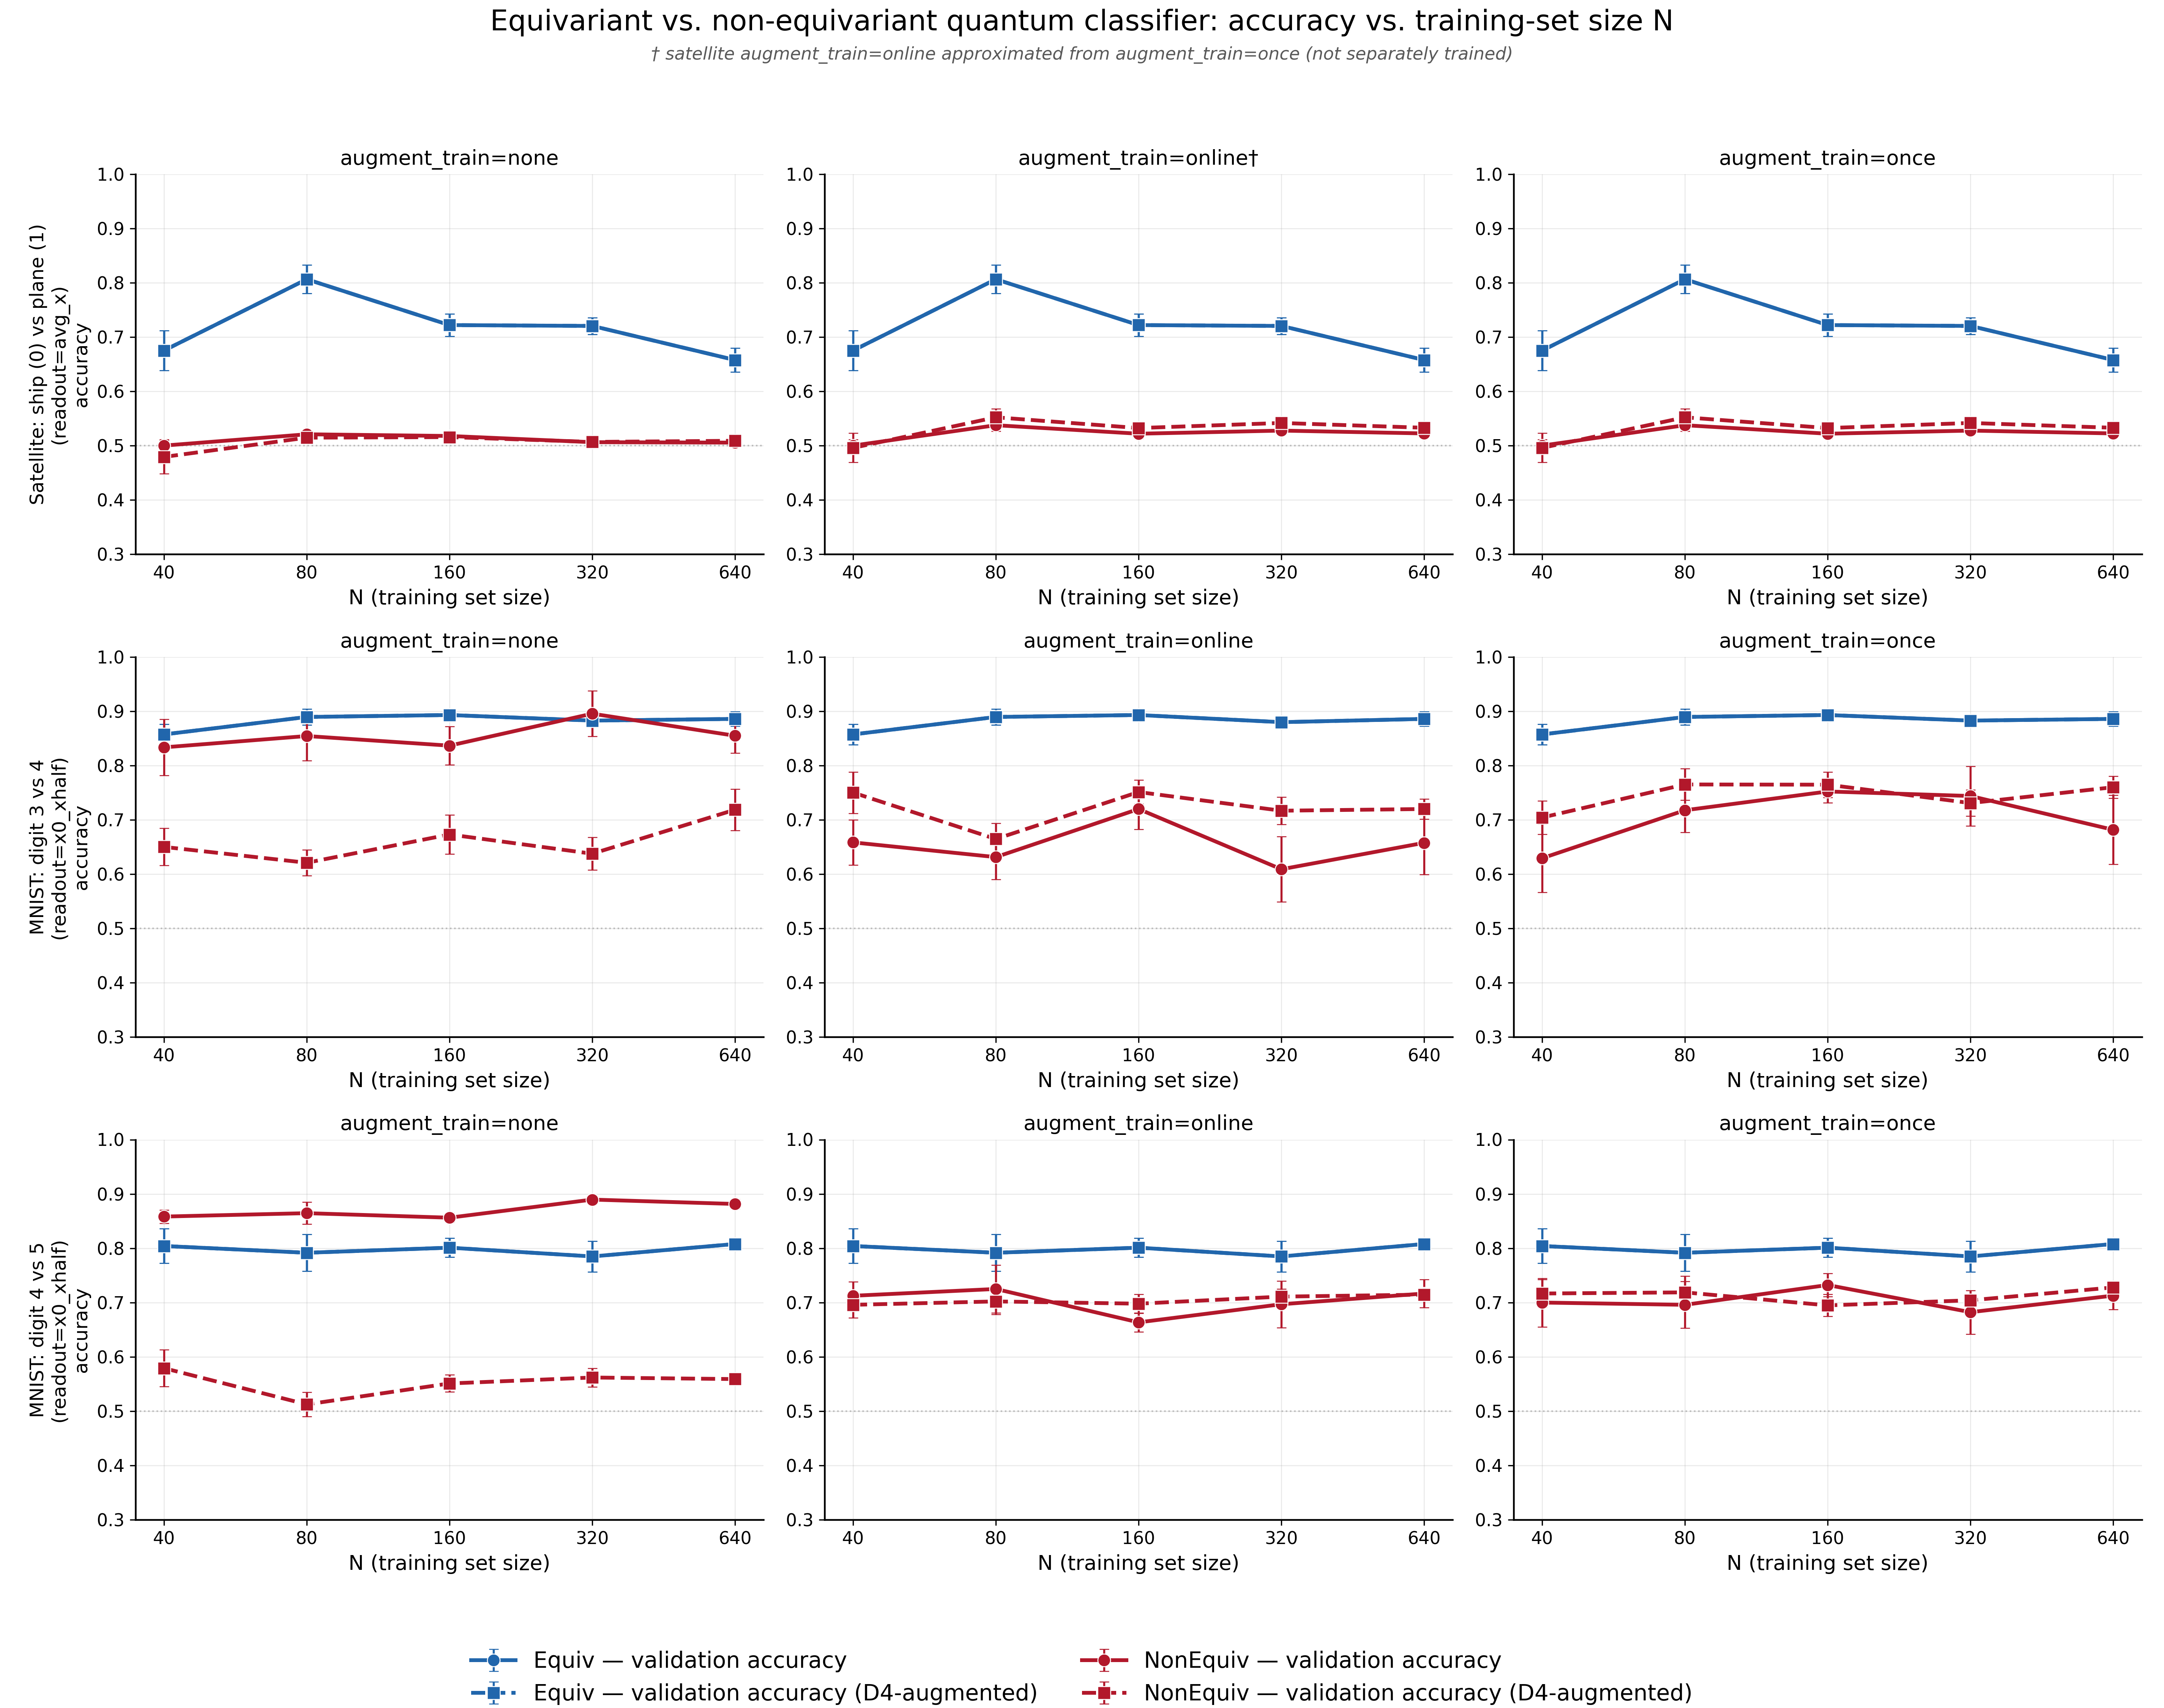
\includegraphics[width=\linewidth]{combined_grid.png}

    \vspace{0.3em}
    {\footnotesize Mean $\pm$ SEM over 6 random seeds. Solid = clean
    validation accuracy; dashed = accuracy on the same images under a
    random $D_4$ (rotation/reflection) transform.
    \dag\ satellite \texttt{augment\_train=online} was not separately
    trained — shown as its \texttt{once} run, which is expected to be
    extremely similar.}
  }

  \block{Conclusion}{
    On a harder, real-world-like task, the practical bottleneck for
    this small (6-parameter) equivariant ansatz was not encoding
    fidelity — a classical model on the same preprocessed input
    recovers most of the discriminative signal — but training length
    and readout choice. Equivariance still delivered its core promise,
    better generalization under symmetry transformations of the
    input, even where raw accuracy on the harder dataset remained well
    below MNIST's.
  }

  \block{Encoding}{
    \centering
    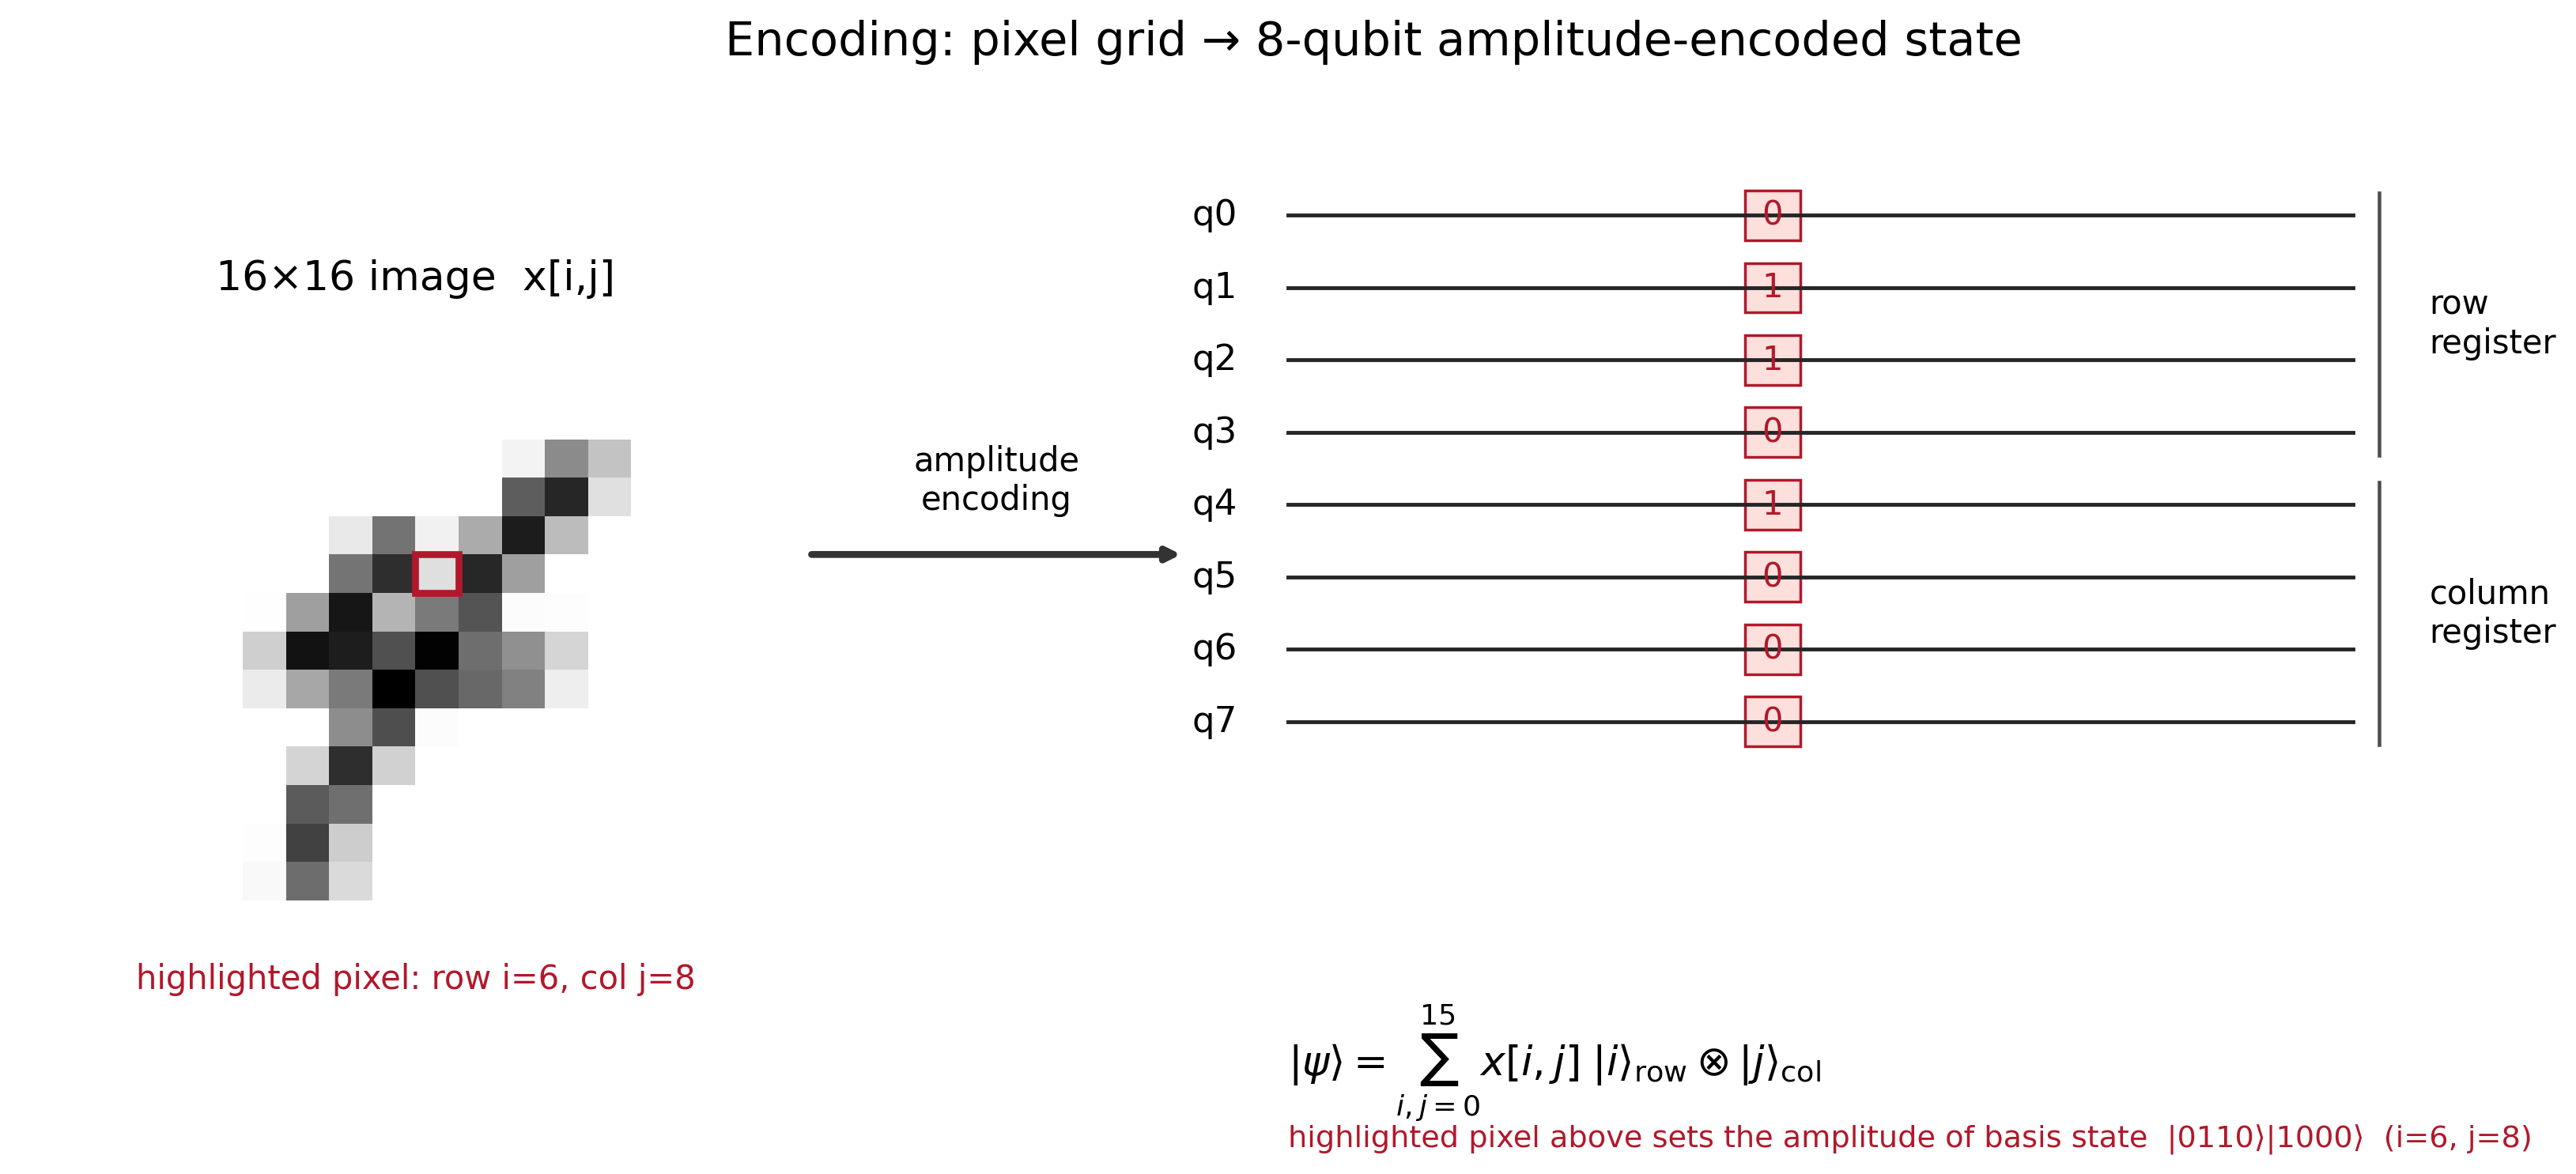
\includegraphics[width=\linewidth]{encoding_diagram.png}
  }

  \block{The two circuits (Equiv, left; NonEquiv, right)}{
    \centering
    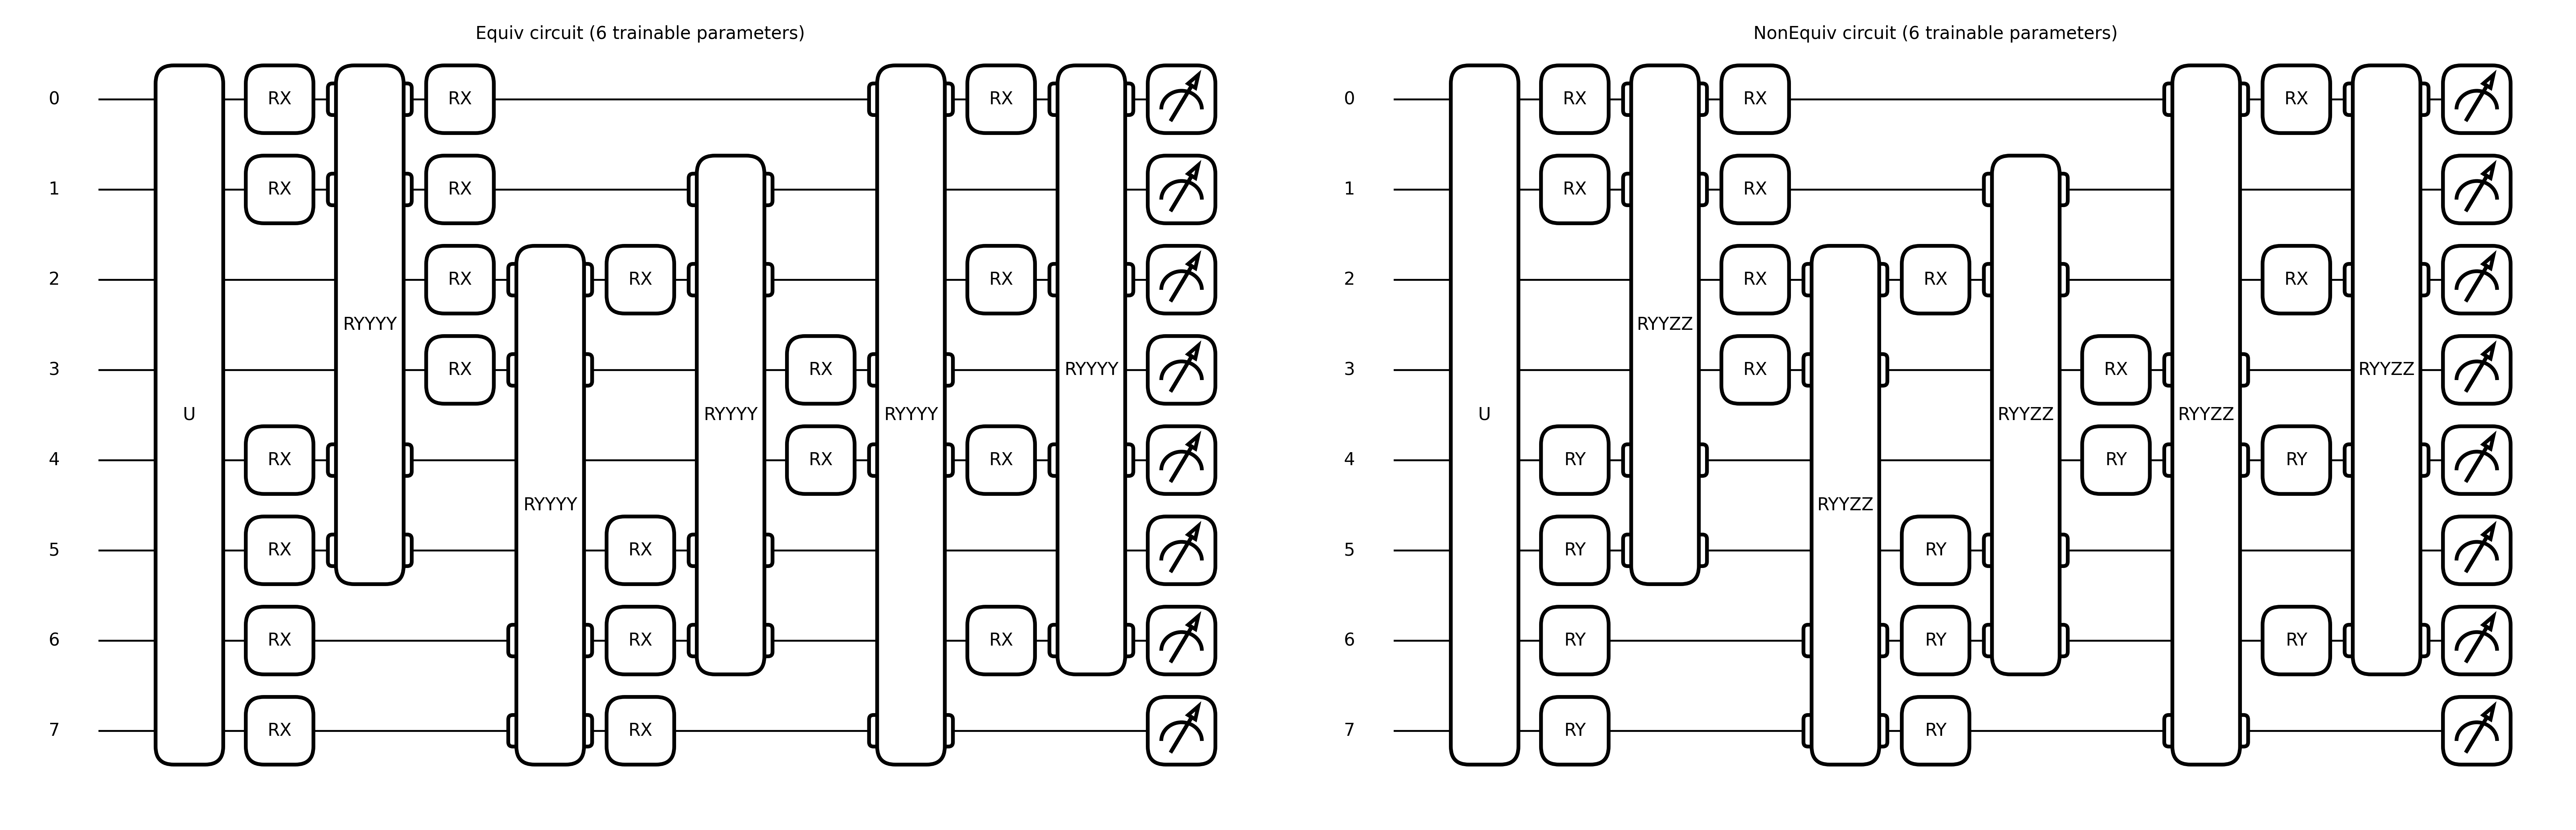
\includegraphics[width=\linewidth]{circuits_side_by_side.png}
  }

  %% ==================================================================
  \column{0.29}

  \block{Datasets}{
    \textbf{MNIST}: two digit pairs (3~vs~4, 4~vs~5), standard
    train/test split.

    \vspace{0.5em}
    \centering
    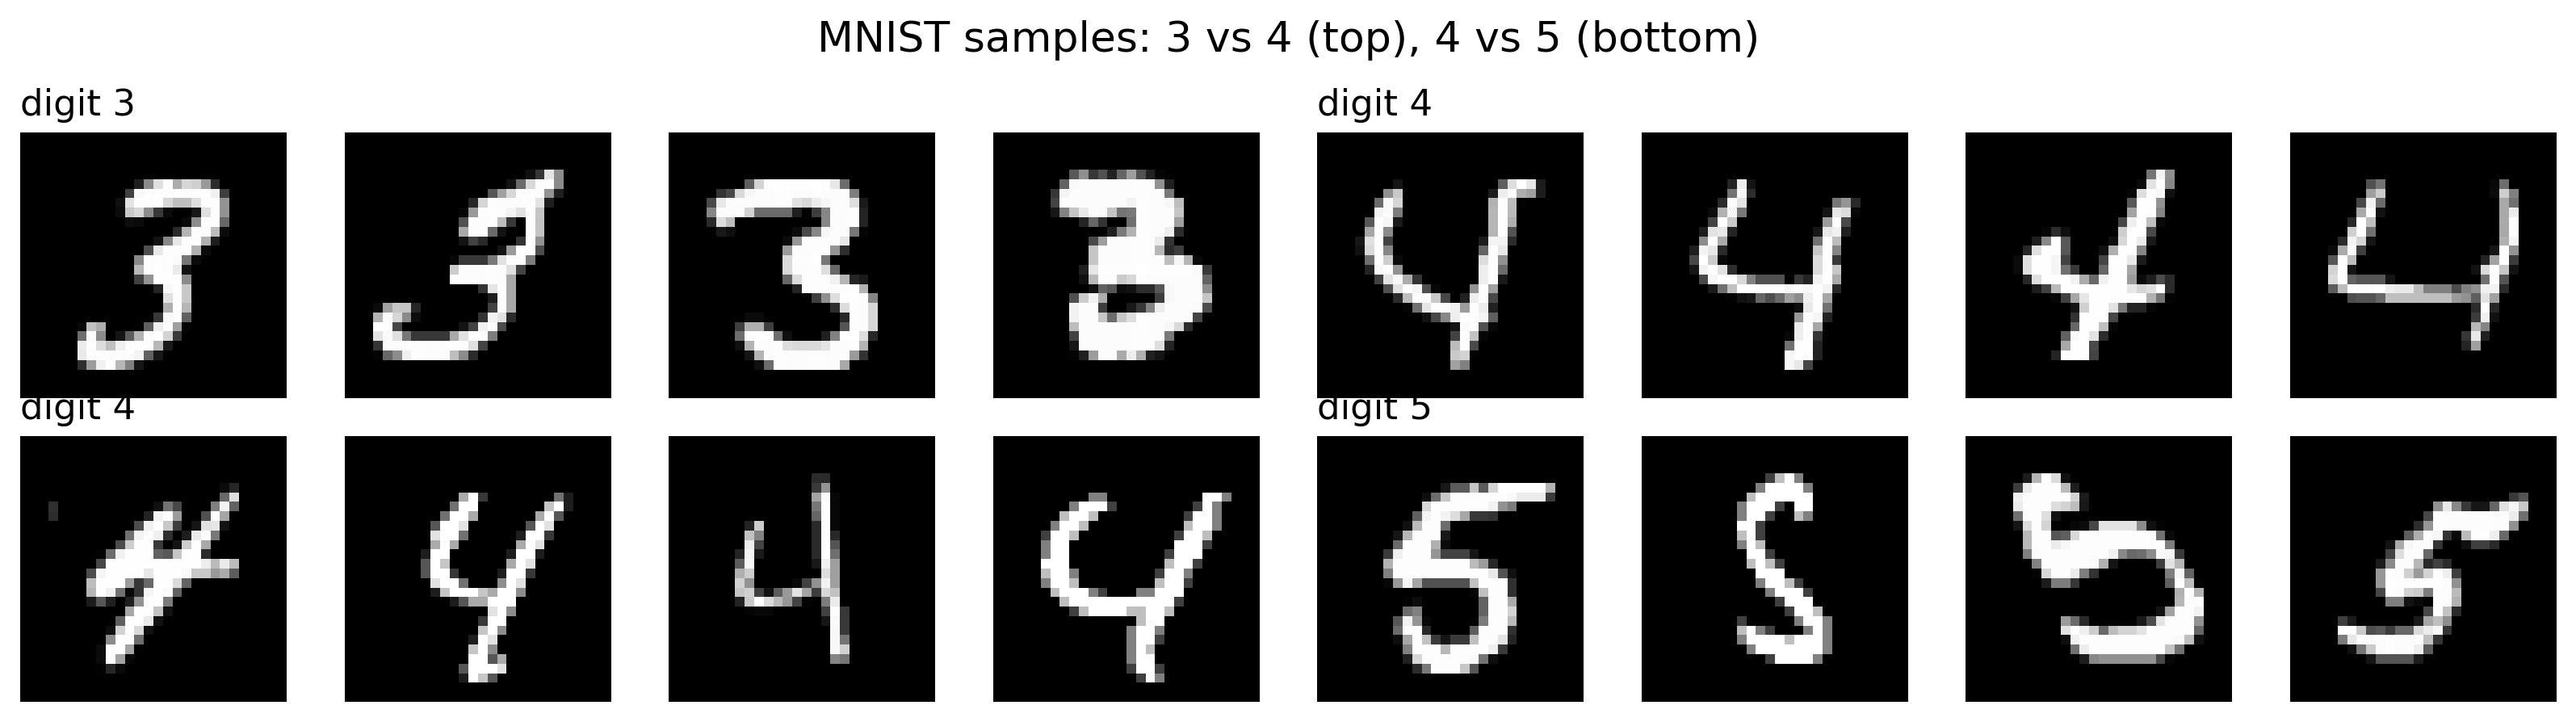
\includegraphics[width=0.95\linewidth]{samples_mnist.png}
    \raggedright

    \vspace{0.8em}
    \textbf{Satellite}: ship
    (\texttt{rhammell/ships-in-satellite-imagery}) vs.\ plane
    (\texttt{rhammell/planesnet}) chips, positive-class images only,
    resized to $16{\times}16$ grayscale.

    \vspace{0.5em}
    \centering
    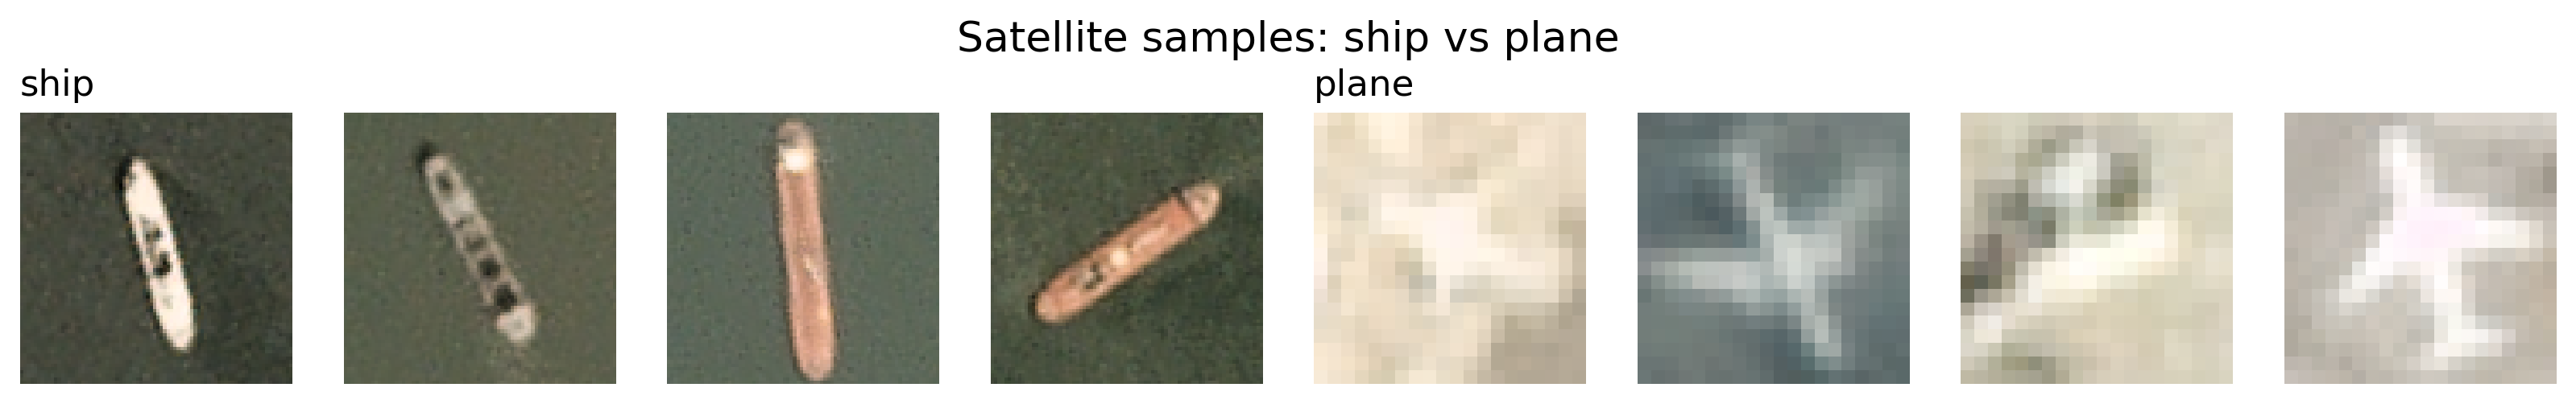
\includegraphics[width=0.95\linewidth]{samples_satellite.png}
    \raggedright

    \vspace{0.8em}
    Each class's images are split once, deterministically, into
    train/test pools \emph{before} any $N$-based sampling, then sampled
    $N/2$-per-class from each pool — guaranteeing exact 50/50 balance
    in both train and test at every $N$ (up to $N{=}1000$, bounded by
    the smaller ships pool of 1000 images).
  }

  \block{Key findings}{
    \begin{itemize}[leftmargin=1.4em]
      \item \textbf{Equivariance buys robustness, not just raw
        accuracy.} Equiv's accuracy on $D_4$-transformed images tracks
        its clean accuracy closely on \emph{both} datasets; NonEquiv's
        drops sharply (e.g.\ MNIST 4~vs~5: $88\%
        \rightarrow 56\%$ under \texttt{augment\_train=none}).

      \item \textbf{The best readout is dataset-dependent.}
        \texttt{x0\_xhalf} wins on MNIST ($\sim\!89\%$);
        \texttt{avg\_x} wins on satellite ($\sim\!72$–$80\%$). A
        per-qubit $\langle X\rangle$ profiling experiment found the
        \emph{same} qubits (0, 2, 4, 6) carry the strongest signal in
        both cases — MNIST's signal is just $\sim\!3\times$ stronger
        overall, so reading only 2 of those qubits is still enough
        there, but not on satellite.

      \item \textbf{Training duration mattered far more than
        expected} on the harder task. At 40 epochs, satellite accuracy
        averaged $65.5\%$ (std $10.5\%$ — two of six seeds still
        near chance); at 70 epochs it reached $74.8\%$ (std
        $0.9\%$). The training \emph{loss} looked flat from
        epoch~$\sim\!10$ while accuracy kept improving for another 60
        epochs — a flat loss does not necessarily mean a flat
        decision boundary.

      \item \textbf{A classical linear baseline} (logistic regression
        on the same preprocessed pixels) reaches
        $80$–$99\%$ on satellite, well above any quantum result
        found — a real, unclosed gap.

      \item \textbf{Naive attempts to close that gap
        underperformed.} Adding 2-qubit entangling gates, doubling or
        tripling circuit depth, and restricting the readout to only
        the empirically-strongest qubits all did \emph{worse} than
        the simple \texttt{avg\_x} baseline.
    \end{itemize}
  }

\end{columns}

\end{document}
